\newpage
\subsection{Caso d'uso UC11: Pagina Utente}
\label{UC11}
\begin{figure}[h]
	\centering
	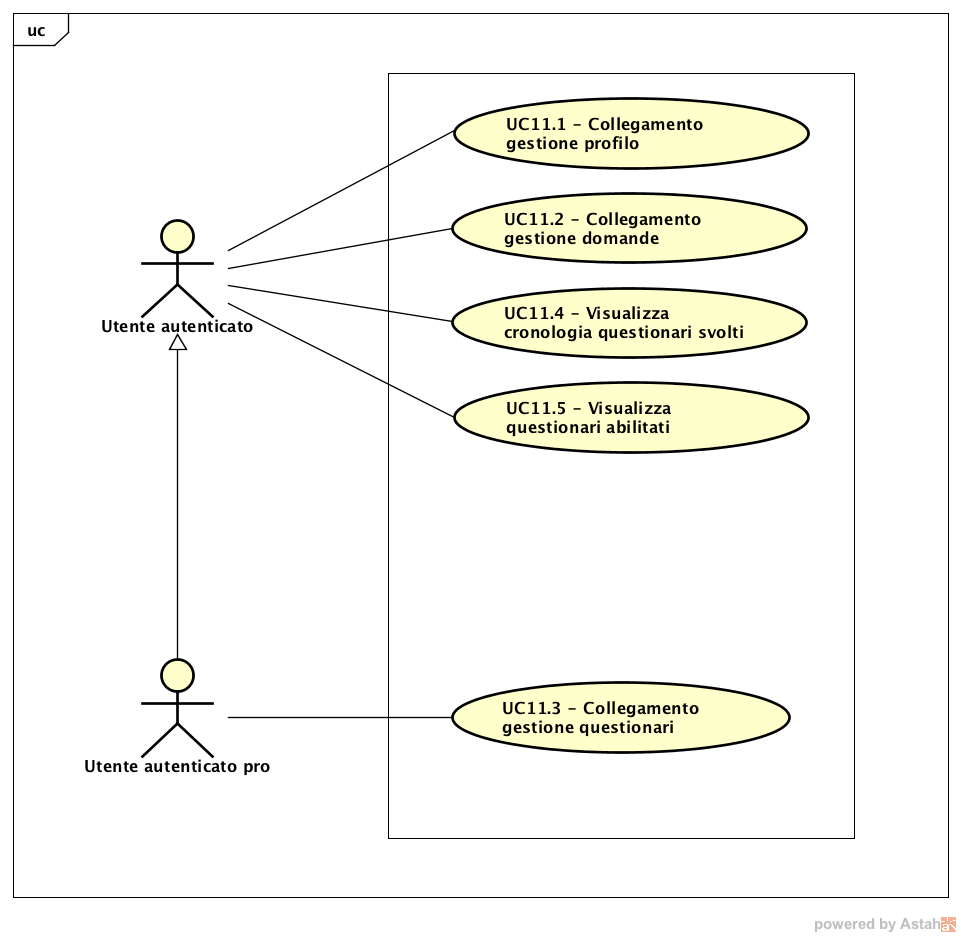
\includegraphics[scale=0.5]{UML/UC11.png}
	\caption{UC11: Gestione pagina utente}
\end{figure}

\begin{itemize}
\item\textbf{Attori}: utente autenticato, utente autenticato pro;
\item\textbf{Descrizione}: l'utente da questa pagina può: 
\begin{itemize}
	\item Visualizzare tutti i dati del suo profilo;
	\item Visualizzare le statistiche dei questionari svolti;
	\item Visualizzare la cronologia dei questionari svolti;
	\item Accedere alla parte del sistema che gli permette di modificare il profilo;
	\item Accedere alla parte del sistema che gli permette di aggiungere nuove domande;
	\item Accedere alla parte del sistema che gli permette di creare questionari.
\end{itemize}
\item\textbf{Precondizione}: l'utente è entrato nella pagina di visualizzazione del profilo;
\item\textbf{Postcondizione}: l'utente ha visualizzato i suoi dati;
\item\textbf{Scenario principale}:
\begin{itemize}
\item L'utente ha scelto di andare alla pagina di gestione del profilo (UC11.1);
\item L'utente ha scelto di andare alla pagina di gestione delle domande (UC11.2);  
\item L'utente ha scelto di andare alla pagina di gestione dei questionari (UC11.3);
\item L'utente ha scelto di andare alla pagina di visualizzazione della cronologia dei questionari svolti (UC11.4);
\item L'utente ha scelto di visualizzazione le statistiche di un questionario (UC11.4.1);
\item L'utente ha scelto di andare alla pagina di visualizzazione dei questionari abilitati (UC11.5);
\item L'utente ha selezionato un questionario abilitato (UC11.5.1);
\end{itemize}
\item\textbf{Inclusioni}: Viene incluso l'UC7 per la compilazione dei questionari.
\end{itemize}

\subsubsection{Caso d'uso UC11.1: Collegamento gestione profilo}
\begin{itemize}
\item\textbf{Attori}: utente autenticato, utente autenticato pro;
\item\textbf{Descrizione}: l'utente viene portato nella pagina di gestione del profilo dove potrà modificare liberamente tutti i suoi dati;
\item\textbf{Precondizione}: l'utente ha premuto l'apposito link di gestione del profilo;
\item\textbf{Postcondizione}: il sistema ha portato l'utente alla pagina di gestione del profilo;
\item\textbf{Scenario principale}: l'utente si trova nella pagina di gestione del profilo e potrà attuare tutte le modifiche desiderate;
\end{itemize}

\subsubsection{Caso d'uso UC11.2: Collegamento gestione delle domande}
\begin{itemize}
\item\textbf{Attori}: utente autenticato, utente autenticato pro;
\item\textbf{Descrizione}: l'utente viene portato nella pagina di gestione delle domande dove potrà inserire o modificare le sue domande;
\item\textbf{Precondizione}: l'utente ha premuto l'apposito link di gestione delle domande;
\item\textbf{Postcondizione}: il sistema ha portato l'utente alla pagina di gestione delle domande;
\item\textbf{Scenario principale}: l'utente si trova nella pagina di gestione delle domande e potrà attuare tutte le modifiche desiderate;
\end{itemize}

\subsubsection{Caso d'uso UC11.3: Collegamento gestione questionari}
\begin{itemize}
\item\textbf{Attori}: utente autenticato, utente autenticato pro;
\item\textbf{Descrizione}: l'utente viene portato nella pagina di gestione dei questionari dove potrà compiere tutte le azioni possbili sui questionari;
\item\textbf{Precondizione}: l'utente ha premuto l'apposito link di gestione dei questionari;
\item\textbf{Postcondizione}: il sistema ha portato l'utente alla pagina di gestione dei questionari;
\item\textbf{Scenario principale}: l'utente si trova nella pagina di gestione dei questionari e potrà attuare tutte le modifiche desiderate;
\end{itemize}

\subsubsection{Caso d'uso UC11.4: Visualizzazione cronologia questionari svolti}
\label{UC11.4}
\begin{figure}[h]
	\centering
	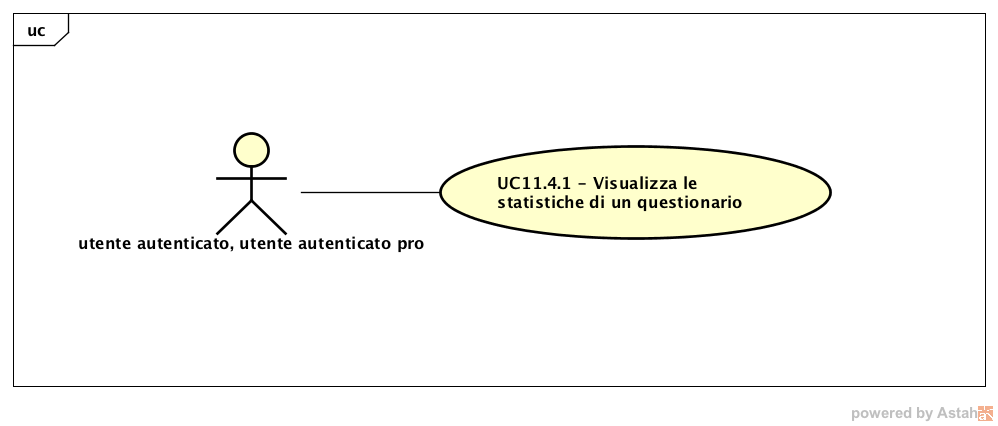
\includegraphics[scale=0.5]{UML/UC11_4.png}
	\caption{UC11.4: Visualizzazione cronologia questionari svolti}
\end{figure}
\begin{itemize}
\item\textbf{Attori}: utente autenticato, utente autenticato pro;
\item\textbf{Descrizione}: 
\item\textbf{Precondizione}:
\item\textbf{Postcondizione}: 
\item\textbf{Scenario principale}: 
\end{itemize}

\subsubsection{Caso d'uso UC11.4.1: Visualizza le statistiche di un questionario scelto}
\begin{itemize}
\item\textbf{Attori}: utente autenticato, utente autenticato pro;
\item\textbf{Descrizione}: 
\item\textbf{Precondizione}:
\item\textbf{Postcondizione}: 
\item\textbf{Scenario principale}: 
\end{itemize}

\subsubsection{Caso d'uso UC11.5: Visualizza questionari abilitati}
\label{UC11.5}
\begin{figure}[h]
	\centering
	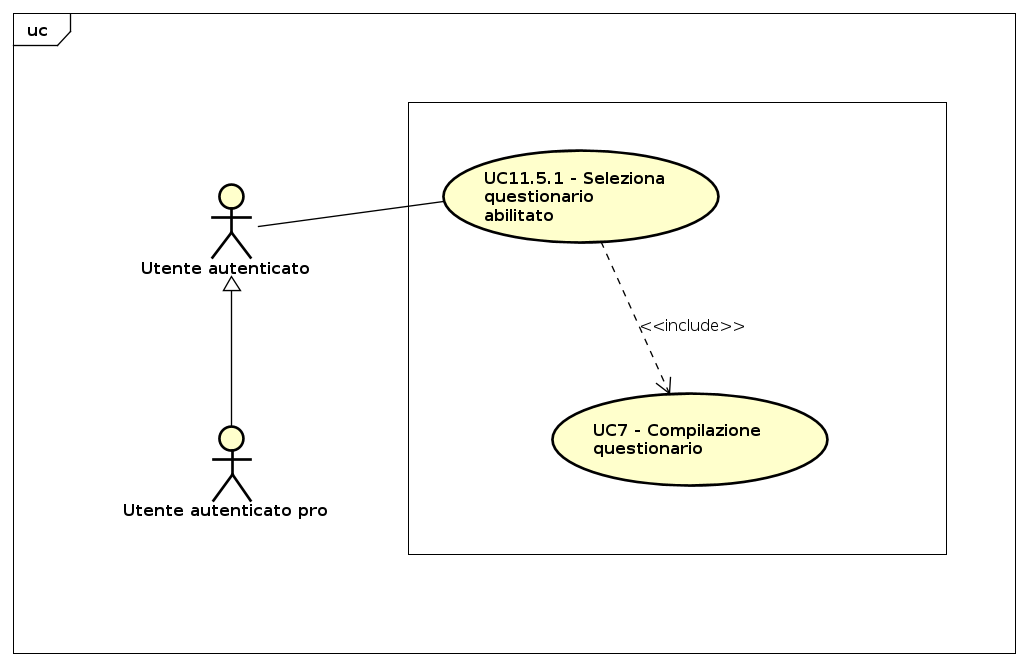
\includegraphics[scale=0.5]{UML/UC11_5.png}
	\caption{UC11.5: Visualizza questionari abilitati}
\end{figure}
\begin{itemize}
\item\textbf{Attori}: utente autenticato, utente autenticato pro;
\item\textbf{Descrizione}: 
\item\textbf{Precondizione}:
\item\textbf{Postcondizione}: 
\item\textbf{Scenario principale}: 
\end{itemize}

\subsubsection{Caso d'uso UC11.5.1: Seleziona questionario abilitato}
\begin{itemize}
\item\textbf{Attori}: utente autenticato, utente autenticato pro;
\item\textbf{Descrizione}: 
\item\textbf{Precondizione}:
\item\textbf{Postcondizione}: 
\item\textbf{Scenario principale}: 
\end{itemize}